\documentclass[12pt]{article}
%Gummi|065|=)
\usepackage{amsmath, amsfonts, amssymb}
\usepackage[margin=0.5in]{geometry}
\usepackage{xcolor}
\usepackage{graphicx}

% zeta functions of cubic fields

%\usepackage{pifont}
\usepackage{amsmath}

\newcommand{\off}[1]{}
\DeclareMathSizes{20}{30}{20}{18}

\usepackage{tikz}

\begin{document}

\sffamily

\fontfamily{qag}\selectfont \fontsize{20}{15}\selectfont

\noindent  \textbf{Diagonal Sudoku} \\\\
\fontfamily{qag}\selectfont \fontsize{15}{15}\selectfont
Each digit  appears exactly once in each of the two main diagonals.  \\ \\
\fontfamily{qag}\selectfont \fontsize{30}{15}\selectfont
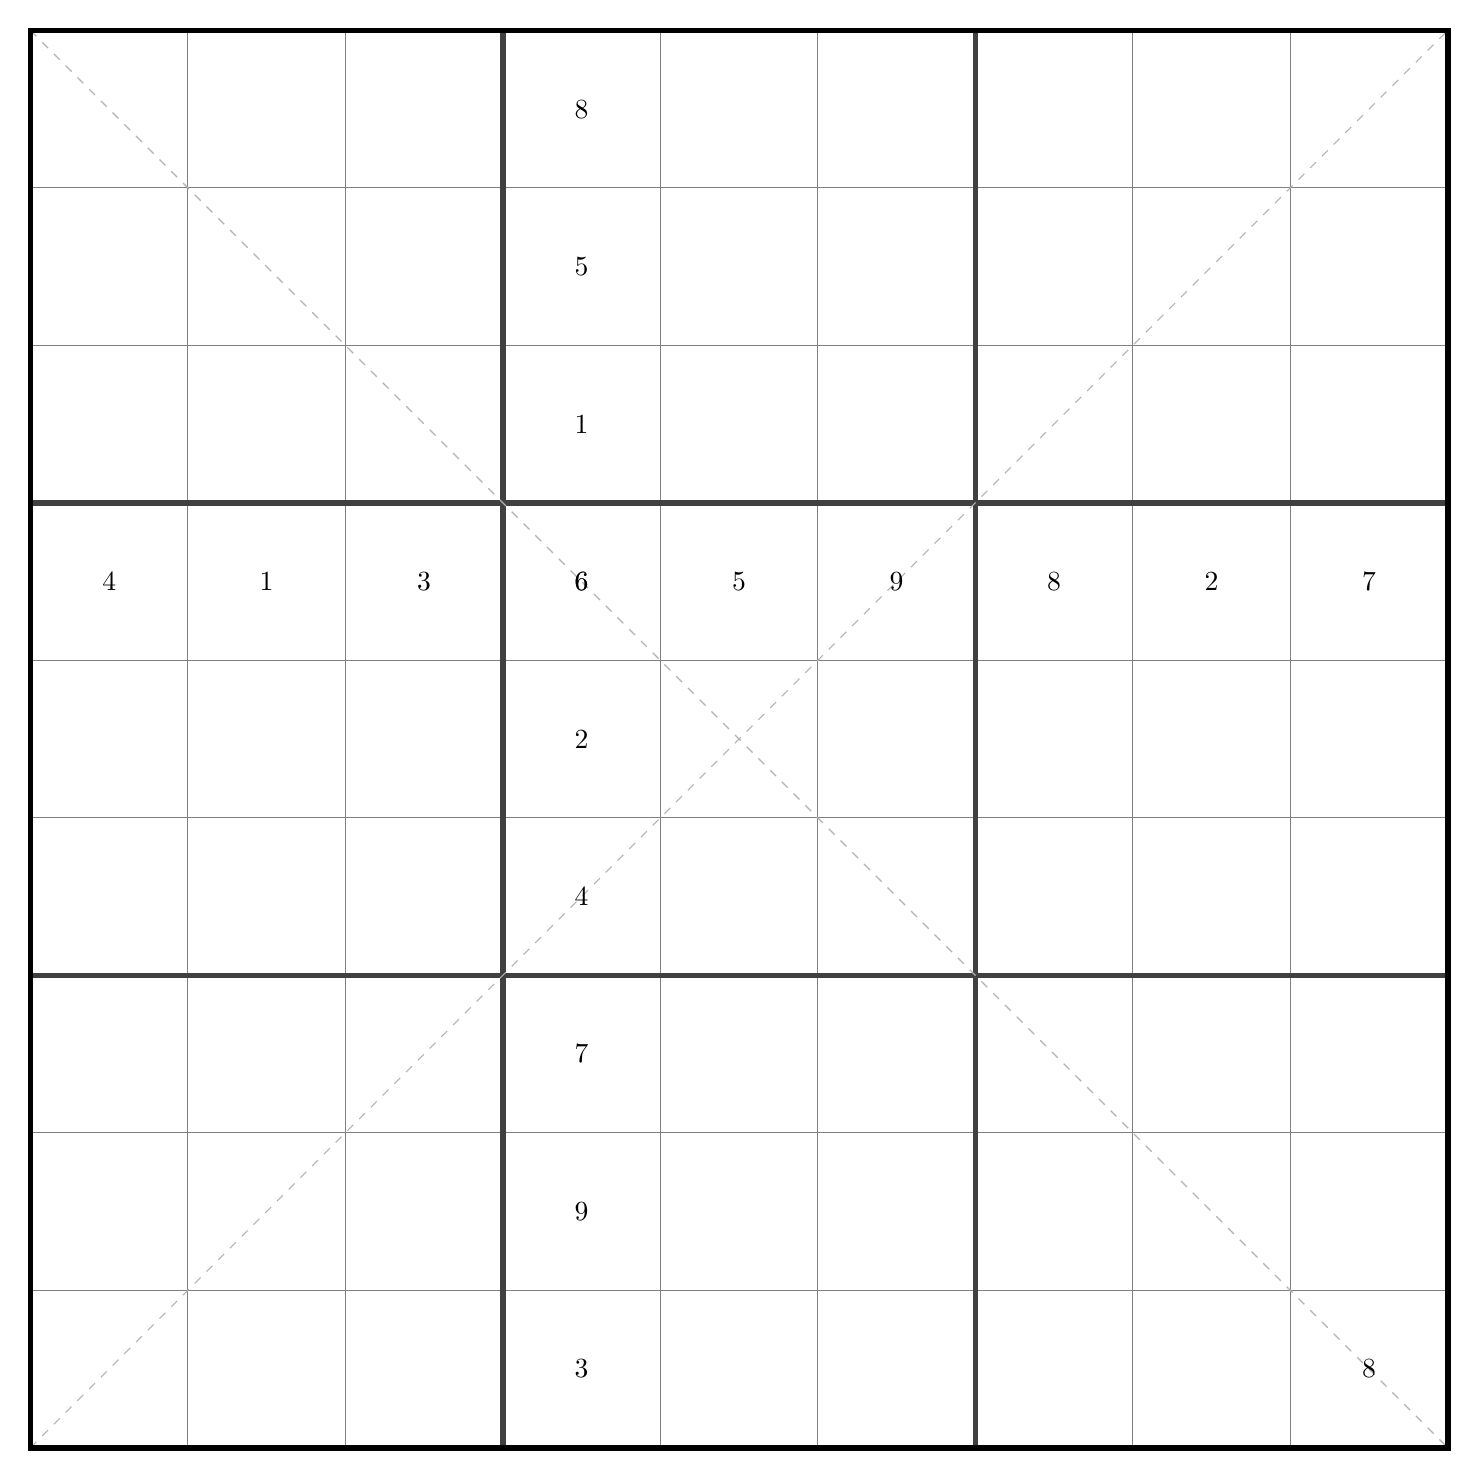
\begin{tikzpicture}[scale=2]

\foreach \a in {1,...,9}{
	\draw[color=black!50!white] (0,\a)--(9,\a);
	\draw[color=black!50!white] (\a,0)--(\a,9);
}

\foreach \a in {0,3,6,9}{
	\draw[color=black!75!white, line width=2] (0,\a)--(9,\a);
	\draw[color=black!75!white, line width=2] (\a,0)--(\a,9);
}

\draw[dashed,color=black!30!white] (0,0)--(9,9);
\draw[dashed,color=black!30!white] (0,9)--(9,0);

\draw[line width = 2] (0,0)--(9,0)--(9,9)--(0,9)--cycle;

\node at (3 + 0.5,8 + 0.5) {8};
\node at (3 + 0.5,7 + 0.5) {5};
\node at (3 + 0.5,6 + 0.5) {1};
\node at (3 + 0.5,5 + 0.5) {6};
\node at (3 + 0.5,4 + 0.5) {2};
\node at (3 + 0.5,3 + 0.5) {4};
\node at (3 + 0.5,2 + 0.5) {7};
\node at (3 + 0.5,1 + 0.5) {9};
\node at (3 + 0.5,0 + 0.5) {3};
\node at (0 + 0.5,5 + 0.5) {4};
\node at (1 + 0.5,5 + 0.5) {1};
\node at (2 + 0.5,5 + 0.5) {3};
\node at (3 + 0.5,5 + 0.5) {6};
\node at (4 + 0.5,5 + 0.5) {5};
\node at (5 + 0.5,5 + 0.5) {9};
\node at (6 + 0.5,5 + 0.5) {8};
\node at (7 + 0.5,5 + 0.5) {2};
\node at (8 + 0.5,5 + 0.5) {7};
\node at (8 + 0.5,0 + 0.5) {8};

\end{tikzpicture} 

\newpage

\fontfamily{qag}\selectfont \fontsize{20}{15}\selectfont

\noindent  \textbf{Outside Sudoku} \\\\
\fontfamily{qag}\selectfont \fontsize{12.5}{15}\selectfont
Follow Classic Sudoku Rules. Digits are given outside of the grid, and each digit must \\ appear in the first region (three cells) in the corresponding row/column.   \\ \\
\fontfamily{qag}\selectfont \fontsize{25}{15}\selectfont
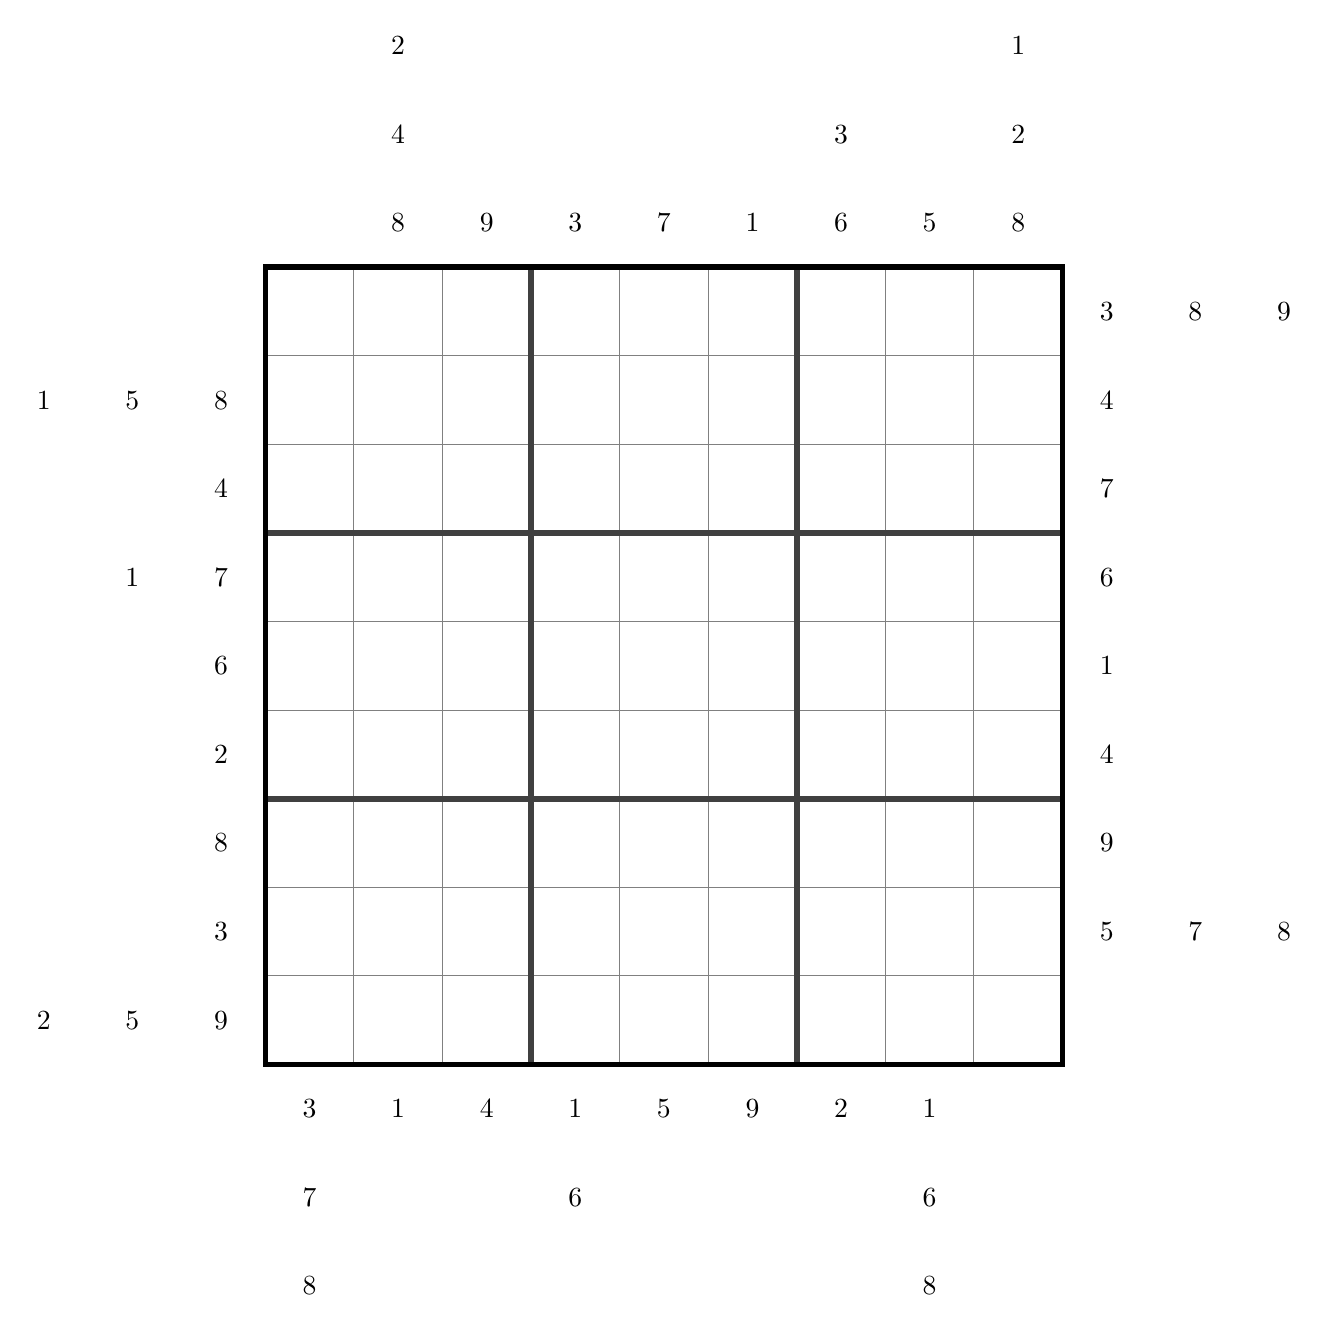
\begin{tikzpicture}[scale=1.125]

\foreach \a in {1,...,9}{
	\draw[color=black!50!white] (0,\a)--(9,\a);
	\draw[color=black!50!white] (\a,0)--(\a,9);
}

\foreach \a in {0,3,6,9}{
	\draw[color=black!75!white, line width=2] (0,\a)--(9,\a);
	\draw[color=black!75!white, line width=2] (\a,0)--(\a,9);
}

%\draw[dashed,color=black!30!white] (0,0)--(9,9);
%\draw[dashed,color=black!30!white] (0,9)--(9,0);

\draw[line width = 2] (0,0)--(9,0)--(9,9)--(0,9)--cycle;

\node at (-3 + 0.5,7 + 0.5) {1};
\node at (-2 + 0.5,7 + 0.5) {5};
\node at (-1 + 0.5,7 + 0.5) {8};
\node at (-1 + 0.5,6 + 0.5) {4};
\node at (-2 + 0.5,5 + 0.5) {1};
\node at (-1 + 0.5,5 + 0.5) {7};
\node at (-1 + 0.5,4 + 0.5) {6};
\node at (-1 + 0.5,3 + 0.5) {2};
\node at (-1 + 0.5,2 + 0.5) {8};
\node at (-1 + 0.5,1 + 0.5) {3};
\node at (-3 + 0.5,0 + 0.5) {2};
\node at (-2 + 0.5,0 + 0.5) {5};
\node at (-1 + 0.5,0 + 0.5) {9};

\node at (9 + 0.5,8 + 0.5) {3};
\node at (10 + 0.5,8 + 0.5) {8};
\node at (11 + 0.5,8 + 0.5) {9};
\node at (9 + 0.5,7 + 0.5) {4};
\node at (9 + 0.5,6 + 0.5) {7};
\node at (9 + 0.5,5 + 0.5) {6};
\node at (9 + 0.5,4 + 0.5) {1};
\node at (9 + 0.5,3 + 0.5) {4};
\node at (9 + 0.5,2 + 0.5) {9};
\node at (9 + 0.5,1 + 0.5) {5};
\node at (10 + 0.5,1 + 0.5) {7};
\node at (11 + 0.5,1 + 0.5) {8};

\node at (0 + 0.5,-1 + 0.5) {3};
\node at (0 + 0.5,-2 + 0.5) {7};
\node at (0 + 0.5,-3 + 0.5) {8};
\node at (1 + 0.5,-1 + 0.5) {1};
\node at (2 + 0.5,-1 + 0.5) {4};
\node at (3 + 0.5,-1 + 0.5) {1};
\node at (3 + 0.5,-2 + 0.5) {6};
\node at (4 + 0.5,-1 + 0.5) {5};
\node at (5 + 0.5,-1 + 0.5) {9};
\node at (6 + 0.5,-1 + 0.5) {2};
\node at (7 + 0.5,-1 + 0.5) {1};
\node at (7 + 0.5,-2 + 0.5) {6};
\node at (7 + 0.5,-3 + 0.5) {8};

\node at (1 + 0.5,11 + 0.5) {2};
\node at (1 + 0.5,10 + 0.5) {4};
\node at (1 + 0.5,9 + 0.5) {8};
\node at (2 + 0.5,9 + 0.5) {9};
\node at (3 + 0.5,9 + 0.5) {3};
\node at (4 + 0.5,9 + 0.5) {7};
\node at (5 + 0.5,9 + 0.5) {1};
\node at (6 + 0.5,10 + 0.5) {3};
\node at (6 + 0.5,9 + 0.5) {6};
\node at (7 + 0.5,9 + 0.5) {5};
\node at (8 + 0.5,11 + 0.5) {1};
\node at (8 + 0.5,10 + 0.5) {2};
\node at (8 + 0.5,9 + 0.5) {8};



\end{tikzpicture} 

\newpage

\fontfamily{qag}\selectfont \fontsize{20}{15}\selectfont

\noindent  \textbf{Roman Numeral Sudoku} \\\\
\fontfamily{qag}\selectfont \fontsize{12.5}{15}\selectfont
Follow Classic Sudoku Rules. Additionally, a clue limits its cell to only those digits whose Roman numeral
representation contains the clue text. For example, you can only enter a 4, 5, 6, 7, or 8 into a cell containing a "V"
clue.   \\ \\
\fontfamily{qag}\selectfont \fontsize{25}{15}\selectfont
\begin{tikzpicture}[scale=2]

\foreach \a in {1,...,9}{
	\draw[color=black!50!white] (0,\a)--(9,\a);
	\draw[color=black!50!white] (\a,0)--(\a,9);
}

\foreach \a in {0,3,6,9}{
	\draw[color=black!75!white, line width=2] (0,\a)--(9,\a);
	\draw[color=black!75!white, line width=2] (\a,0)--(\a,9);
}

%\draw[dashed,color=black!30!white] (0,0)--(9,9);
%\draw[dashed,color=black!30!white] (0,9)--(9,0);

\draw[line width = 2] (0,0)--(9,0)--(9,9)--(0,9)--cycle;

\node at (0 + 0.5,8 + 0.5) {IV};
\node at (0 + 0.5,7 + 0.5) {VI};
\node at (0 + 0.5,6 + 0.5) {VII};
\node at (0 + 0.5,5 + 0.5) {III};
\node at (0 + 0.5,4 + 0.5) {II};
\node at (0 + 0.5,3 + 0.5) {I};
\node at (0 + 0.5,2 + 0.5) {X};
\node at (0 + 0.5,1 + 0.5) {II};
\node at (0 + 0.5,0 + 0.5) {V};
\node at (1 + 0.5,8 + 0.5) {IX};
\node at (2 + 0.5,8 + 0.5) {I};
\node at (3 + 0.5,8 + 0.5) {II};
\node at (4 + 0.5,8 + 0.5) {V};
\node at (5 + 0.5,8 + 0.5) {VI};
\node at (6 + 0.5,8 + 0.5) {V};
\node at (7 + 0.5,8 + 0.5) {I};
\node at (8 + 0.5,8 + 0.5) {I};
\node at (8 + 0.5,7 + 0.5) {III};
\node at (8 + 0.5,6 + 0.5) {V};
\node at (8 + 0.5,5 + 0.5) {I};
\node at (8 + 0.5,4 + 0.5) {V};
\node at (8 + 0.5,3 + 0.5) {IX};
\node at (8 + 0.5,2 + 0.5) {V};
\node at (8 + 0.5,1 + 0.5) {IV};
\node at (8 + 0.5,0 + 0.5) {I};
\node at (1 + 0.5,0 + 0.5) {I};
\node at (2 + 0.5,0 + 0.5) {IV};
\node at (3 + 0.5,0 + 0.5) {V};
\node at (4 + 0.5,0 + 0.5) {III};
\node at (5 + 0.5,0 + 0.5) {V};
\node at (6 + 0.5,0 + 0.5) {I};
\node at (7 + 0.5,0 + 0.5) {I};
\node at (3 + 0.5,5 + 0.5) {V};
\node at (3 + 0.5,3 + 0.5) {I};
\node at (5 + 0.5,5 + 0.5) {IX};
\node at (5 + 0.5,3 + 0.5) {VIII};
\node at (2 + 0.5,6 + 0.5) {VII};
\node at (6 + 0.5,2 + 0.5) {VI};
\node at (2 + 0.5,2 + 0.5) {V};
\node at (6 + 0.5,6 + 0.5) {V};
\node at (4 + 0.5,4 + 0.5) {VI};
\node at (3 + 0.5,4 + 0.5) {II};
\node at (4 + 0.5,5 + 0.5) {III};
\node at (4 + 0.5,3 + 0.5) {VI};
\node at (5 + 0.5,4 + 0.5) {I};
\node at (1 + 0.5,7 + 0.5) {V};
\node at (7 + 0.5,1 + 0.5) {V};
\node at (7 + 0.5,7 + 0.5) {IX};
\node at (1 + 0.5,1 + 0.5) {VIII};
\node at (2 + 0.5,7 + 0.5) {II};
\node at (1 + 0.5,6 + 0.5) {II};
\node at (7 + 0.5,2 + 0.5) {V};
\node at (6 + 0.5,1 + 0.5) {II};
\node at (1 + 0.5,2 + 0.5) {I};
\node at (2 + 0.5,1 + 0.5) {V};
\node at (6 + 0.5,7 + 0.5) {I};
\node at (7 + 0.5,6 + 0.5) {IV};
\node at (1 + 0.5,5 + 0.5) {V};
\node at (1 + 0.5,4 + 0.5) {V};
\node at (1 + 0.5,3 + 0.5) {V};
\node at (2 + 0.5,5 + 0.5) {II};
\node at (2 + 0.5,4 + 0.5) {IX};
\node at (2 + 0.5,3 + 0.5) {V};
\node at (6 + 0.5,5 + 0.5) {V};
\node at (6 + 0.5,4 + 0.5) {VI};
\node at (6 + 0.5,3 + 0.5) {II};
\node at (7 + 0.5,5 + 0.5) {VI};
\node at (7 + 0.5,4 + 0.5) {VI};
\node at (7 + 0.5,3 + 0.5) {II};
\node at (3 + 0.5,7 + 0.5) {VI};
\node at (4 + 0.5,7 + 0.5) {I};
\node at (5 + 0.5,7 + 0.5) {I};
\node at (3 + 0.5,6 + 0.5) {I};
\node at (4 + 0.5,6 + 0.5) {IX};
\node at (5 + 0.5,6 + 0.5) {III};
\node at (3 + 0.5,2 + 0.5) {II};
\node at (4 + 0.5,2 + 0.5) {V};
\node at (5 + 0.5,2 + 0.5) {II};
\node at (3 + 0.5,1 + 0.5) {I};
\node at (4 + 0.5,1 + 0.5) {I};
\node at (5 + 0.5,1 + 0.5) {V};

​





\end{tikzpicture}



\end{document}